% fig03_hover_field — Stage-1 hover on-axis field B_z(zeta) for 3 pilot coils.
% Standalone pgfplots; compiled to figures/fig03_hover_field.pdf.
% Comparison (3 coil radii a, same B=2T center) => chart (commons comparison rule).
% Data: Appendix A, UFO/verify/stage1-hover-fields.md.
%   B_z(a,I,zeta) = mu0*I*a^2 / (2*(a^2+zeta^2)^1.5), mu0=4*pi*1e-7
%   coil A: a=0.3 I=954930  -> center 2T
%   coil B: a=0.5 I=1591549 -> center 2T
%   coil C: a=1.0 I=3183099 -> center 2T
\documentclass[border=4pt]{standalone}
\usepackage{tikz}
\usepackage{pgfplots}
\pgfplotsset{compat=1.18}
\begin{document}
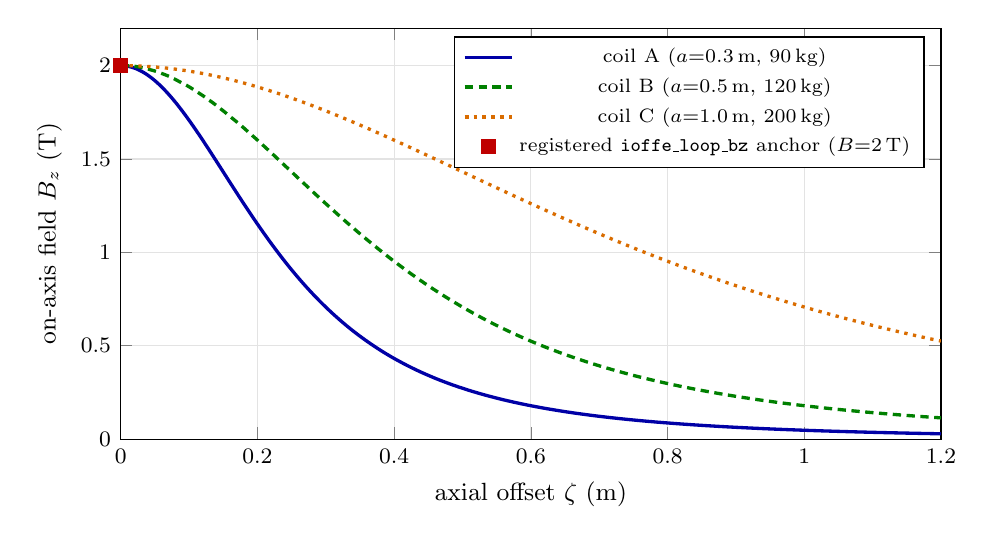
\begin{tikzpicture}
\begin{axis}[
  width=12cm, height=6.8cm,
  xlabel={axial offset $\zeta$ (m)},
  ylabel={on-axis field $B_z$ (T)},
  domain=0:1.2, samples=160,
  xmin=0, xmax=1.2, ymin=0, ymax=2.2,
  tick label style={font=\footnotesize},
  label style={font=\small},
  ymajorgrids, xmajorgrids, grid style={gray!22},
  legend style={font=\scriptsize, at={(0.98,0.98)}, anchor=north east},
]
% mu0/(2) folded numerically into I to hit 2T at zeta=0; use exact loop shape
% B_z = 2 * a^3 / (a^2+zeta^2)^1.5  (since center 2T => B = 2 * a^3/(a^2+z^2)^1.5)
\addplot[blue!65!black, very thick, smooth] {2*0.3^3/(0.3^2+x^2)^1.5};
\addlegendentry{coil A ($a{=}0.3$\,m, 90\,kg)}
\addplot[green!50!black, very thick, smooth, densely dashed] {2*0.5^3/(0.5^2+x^2)^1.5};
\addlegendentry{coil B ($a{=}0.5$\,m, 120\,kg)}
\addplot[orange!85!black, very thick, smooth, dotted] {2*1.0^3/(1.0^2+x^2)^1.5};
\addlegendentry{coil C ($a{=}1.0$\,m, 200\,kg)}
\addplot[only marks, mark=square*, mark size=2.6pt, red!75!black] coordinates {
  (0,2.0)
};
\addlegendentry{registered \texttt{ioffe\_loop\_bz} anchor ($B{=}2$\,T)}
\end{axis}
\end{tikzpicture}
\end{document}
